% abthmsnp.tex
% Application-Based TCP Hijacking
% Author: Oliver Zheng / Jason Poon / Konstantin Beznosov

\documentclass{sig-alternate}

\begin{document}

% --- Metadata ---
\conferenceinfo{EUROSEC}{'09 Nuremberg, Germany}
\CopyrightYear{2009}
\crdata{978-1-60558-472-0/09/0003}
% --- End Metadata ---

\title{
Application-Based TCP Hijacking
}

\numberofauthors {1}
\author {
	\hspace{1.0cm} Oliver Zheng \hspace{3.4cm} Jason Poon \hspace{2.4cm}  Konstantin Beznosov\\
	\email{skillzer@interchange.ubc.ca \hspace{.5cm} jasazn@interchange.ubc.ca \hspace{.5cm} beznosov@ece.ubc.ca}\\
	\vspace{0.1cm}\\
	\affaddr{University of British Columbia}\\
	\affaddr{2332 Main Mall, Vancouver, Canada V6P 3V2}\\
}

\date{\today}

\maketitle

\begin{abstract}
We present application-based TCP hijacking (ABTH), a new attack on TCP applications that exploits flaws due to the interplay between TCP and application protocols to inject data into an application session without either server or client applications noticing the spoofing attack. 
Following the injection of a TCP packet, ABTH resynchronizes the TCP stacks of both the server and the client.
To evaluate the feasibility and effectiveness of ABTH, we developed a tool that allows impersonating users of Windows Live Messenger in the matter of few seconds. 
Due to its generic nature, ABTH can be mounted on a variety of modern protocols for TCP-based applications.
Countermeasures to thwart and/or limit the effectiveness of ABTH could include strict Ethernet switching and cryptographic protection of messages.
However, the former cannot be guaranteed by the application provider and the latter appears to be still prohibitively expensive for such large-scale applications with hundreds of millions of sporadic users as Windows Live Messenger.
\end{abstract}

\terms{Security, Theory}

\keywords{TCP hijacking, application-based TCP hijacking, Windows Live Messenger, application protocols, packet injection}

\section{Introduction}

Since its first specification in 1974~\cite{rfc:tcp}, the Transmission Control Protocol (TCP) has grown to become the core transport protocol for a vast number of applications including HTTP, FTP, SMTP, and TELNET.
The security properties of these application protocols are partially dependent on the security of TCP and the underlying Internet Protocol (IP).
Many network attacks that exploit vulnerabilities of the TCP design have shown prominence over the past decades~\cite{harris:tcpattacks}.
While preventive mechanisms have been developed to throttle or outright eliminate most of these attacks~\cite{dubrawsky:layer2}, the list of TCP vulnerabilities continues to grow.

In this paper, we present application-based TCP hijacking (ABTH), a new technique for attacking TCP-based communications.
ABTH extends TCP hijacking~\cite{stamp:infosec} by meddling with application-layer protocols.
Traditional TCP hijacking attacks exploit vulnerabilities of the transport and network layers.
However, the majority of these attacks have been circumvented through the use of hardware switches and routers~\cite{dubrawsky:layer2}, which provide countermeasures against such direct low-level attacks.
On the other hand, ABTH utilizes loopholes in the logistics of application-level communication to evade policy enforcement at the transport and IP layers.
Trivial design features of application protocols become fatal vulnerabilities that can be exploited by ABTH.

\begin{sloppypar}
To demonstrate the feasibility and effectiveness of ABTH, we developed an attack on the communications of Microsoft Windows Live Messenger (WLM).
With instant messaging (IM) becoming ubiquitous at both home and work~\cite{aol:survey}, Windows Live Messenger (WLM) represents one of the largest IM networks, featuring 17 million users~\cite{microsoft:advertising}.
By attacking the Microsoft Notification Protocol (MSNP)---the protocol in use by WLM---with ABTH, the privacy and confidentiality of WLM users can be compromised; an attacker is capable of spoofing any command available to the WLM client and impersonating any contact known to the victim.
As a result, unauthorized messages can be delivered to various WLM clients.
We contacted Microsoft about the weakness of MSNP against ABTH in the spring of 2008; the subject matter was still under investigation as of February 2009.
Although our sample attack is limited to WLM, due to its generic nature, ABTH can be mounted on a variety of application protocols.
\end{sloppypar}

Among several ways to mitigate ABTH, Internet service providers (ISPs) could employ stricter security controls on the network layer.
TCP applications could also employ TLS or other forms of data confidentiality and integrity protection.
However, the former cannot be guaranteed by the application provider(s) and the latter appears to be still prohibitively expensive for such large-scale applications with millions of sporadic users as WLM.

The remainder of the paper is organized as follows.
Relevant background information on TCP and existing attacks on the transport protocol are discussed in Section~\ref{sec:background}.
The theory and general operation of ABTH is described in Section~\ref{sec:abth}.
The application of ABTH for MSNP is demonstrated in Section~\ref{sec:casestudy}.
The limitations of ABTH and countermeasures against it as well as its feasibility are discussed in Section~\ref{sec:discussion}.
The paper is concluded in Section~\ref{sec:conclusion}.

\section{Background and Related Work}
\label{sec:background}

In this section, necessary background information on TCP including the details of existing security flaws are presented.

\subsection{Overview of TCP}

TCP is a connection-oriented transport protocol that guarantees reliable in-order delivery of network packets~\cite{rfc:tcp}.
A pair of hosts initiate contact and communicate by sending packets to each other.
Each end of the connection is identified by an Internet Protocol (IP) address and a TCP port, both of which are determined prior to the establishment of connection.

Each TCP packet is tagged with a sequence number, an acknowledgement number, and a receive window, herein referred to as seqnum, acknum, and rcvwnd, respectively.
Seqnum represents the n-th byte of data transferred; acknum confirms the n-th byte of data received; rcvwnd corresponds to the number of bytes the host is willing to receive and capable of processing.
Within each TCP header are also 8 control flags.
After a connection is established (which is the only relevant timeframe ABTH deals with), each packet can confirm reception of data by setting the ACK flag and/or contain data; thus, some packets with no data have just the ACK flag set to denote an empty acknowledgement packet.
For each data packet that is sent, a returning packet has to be received with acknum equal the seqnum + the length of the sent packet to affirm delivery of all consecutive bytes up to and including the last byte.
A data packet with the same acknum may be received in lieu of an empty acknowledgement packet, in which case this packet needs confirmation as well.

In order for the two hosts to be in a synchronized state where data packets can be received and processed as valid packets, the seqnum of one host must match the acknum of the other and vice versa. 
As an example to illustrate seqnum and acknum, a client connects to a server through TCP.
After establishing a connection, assume the client has a seqnum of 50 and the server has a seqnum of 100.
The next packet the client sends must entail seqnum 50 and acknum 100.
If the client sends a data packet of 10 bytes, the client seqnum increases to 60 and the server must send an acknowledgement packet with seqnum 100 and acknum 60.

When either hosts receives a packet containing an unexpected seqnum two scenarios may occur.
If the received seqnum is within the range of the expected seqnum and the rcvwnd (the received packet arrived before another packet with the expected seqnum), the data is buffered and no acknowledgement packet is sent.
(An acknowledgement packet would confirm the reception of the missing packet.)
Otherwise, the packet is dropped and an acknowledgement packet is sent with an acknum of the expected seqnum, which may incite a TCP ack storm~\cite{joncheray:1995}, an undesirable effect in the perspective of an attacker.

\subsection{Adversary Model}
\label{sec:adversarymodel}

For the TCP attacks to follow as well as ABTH, the main assumption is that attackers are able to listen to network traffic of a TCP session and inject spoofed packets into the network.
We do not assume that the attacker has necessarily the capabilities of launching a denial-of-service attack or deleting or rerouting network traffic.
Additionally, the attacker is assumed not to need to temper with the establishing of the TCP connection; the attacker may administer an attack on any live TCP connection anytime.

In wired networks, sniffing and spoofing may be very limited.
For example, network switches prevent sniffing in Ethernet and it is usually very difficult to sniff on routers.
Internet service providers (ISPs) and enterprises often use network access control to block IP spoofing.
However, in wireless networks, especially in unencrypted 802.11 networks, sniffing and spoofing can be done with well designed software and off-the-shelf hardware.

Computational capabilities of the attacker do not go beyond the limits of a consumer-level personal computer.
For example, in our implementation of ABTH for Windows Live Messenger, the victim was attacked in the matter of two seconds with the use of a modest laptop.

\subsection{Attacks on TCP}

Many attacks on TCP exploit vulnerabilities of the seqnum and acknum synchronization mechanism.
In order to demonstrate the value of ABTH, attacks pertinent to ABTH are first discussed in the following sections.
All of these attacks, including ABTH, assume the threat model defined in Section~\ref{sec:adversarymodel}.
There are other TCP attacks that assume different (and perhaps weaker) adversary models, but they are not relevant for this discussion.

\subsubsection{TCP Hijacking}

By eavesdropping on a TCP session, an attacker is able to observe and calculate the expected seqnums and acknums of both hosts and is therefore able to inject a spoofed TCP packet~\cite{harris:tcpattacks}.
The spoofed packet would contain the seqnum and acknum expected by the recipient and the source address of the other host.
Although the spoofed packet is sent by the attacker, the recipient does not have the ability to authenticate the source of the packet and would therefore accept it as a valid packet.
However, following this spoof, the connection is effectively broken, as the expected seqnums and acknums of the two hosts are out of sync.
Subsequent data packets sent to either host would be regarded as invalid due to the mismatch of numbers, and no acknowledgement packets are sent in response.
Thus, the connection is quickly reset by both hosts.
As a result, both hosts would notice a disruption in the network service and may suspect an attack.

\subsubsection{Man-in-the-Middle}

Following a TCP hijacking attack, the attacker can act as a man-in-the-middle by relaying all messages from one host to the other~\cite{joncheray:1995, gregg:stackhack}.
Although the initial spoofed packet has caused an imbalance between the TCP stacks of both hosts, for each packet sent by either hosts, an attacker is able to forward the packet to the recipient host by spoofing a copy of the packet and translating the seqnums and acknums on the fly.
However, a problem arises when each host receives the original packet(s) that was sent to each other, with the unexpected seqnums and acknums.
As previously mentioned, a packet is considered valid if its seqnum falls within the range of the expected seqnum and the rcvwnd.
Spoofed packets cause the spoofed host to lag behind on its seqnum, and thus packets sent from the spoofed host are not in the acceptable range.
Subsequently, for each packet the spoofed host sends, the other host drops it and sends back an acknowledgement packet with the expected seqnum and acknum trying to correct this desynchronization.
The spoofed host would try to do the same by sending an acknowledgement packet, which incites the other host to send another.
This repeated cycle of sending packets creates an ack storm, in which both hosts continuously send empty ack packets.

While the ack storm stops as soon as one packet is dropped due to the unreliability of the underlying physical network, it creates a massive load of network traffic~\cite{joncheray:1995}.
Intrusion detection systems can characterize this load with statistical analysis of empty packets on the network and notify users of the attack.

\subsubsection{ARP Poisoning}

A method of avoiding TCP ack storms is to stop hosts from receiving legitimate packets.
While the attacker cannot delete or reroute packets, the attacker can utilize Address Resolution Protocol (ARP) poisoning to mislead hosts into ignoring legitimate packets.
ARP provides translation of IP address to MAC address.
If ARP poisoned with the wrong MAC address, a host will send TCP/IP packets to the wrong MAC address and ignore incoming packets from the real MAC address.
The attacker needs only to poison ARP tables of one host to circumvent ack storms, as the compromised host will not respond to the other host.

However, ARP traffic does not travel beyond the local area network (LAN) and imposes the restriction that the attacker be within the same LAN as at least one host.
More importantly, ARP poisoning is a low network level attack that can be easily prevented with hardware enforcement~\cite{spangler:sniffing}; most hardware switches disable ARP poisoning.

\subsubsection{Restoring Synchronization}

The attacker can try to resynchronize both hosts by inciting the lagging host to send packets manually~\cite{lam:resync}.
For example, an attacker exploiting the TELNET protocol may send a notice to the user to type in a few characters.
However, slightly more experienced users will easily detect such a peculiarity.

As discussed, existing attacks on TCP do not provide much guarantee for an attack to be executed unnoticed.

\section{Application-Based TCP Hijacking}
\label{sec:abth}

ABTH improves upon conventional TCP session hijacking by allowing an attacker to automatically resynchronize TCP seqnums and acknums of the two hosts of the connection.
It is a specific method of exercising TCP hijacking based on the application protocol without utilizing ARP poisoning or any other techniques below the transport layer.
The technique assumes the adversary model described in Section~\ref{sec:adversarymodel}. 

Many application protocols intended for two-way communication, such as TELNET and FTP, maintain a persistent TCP connection.
A typical method for ensuring the connection is open is for one of the hosts to periodically send an application-level command to the other host.
Application-level commands, such as a ping, feature two characteristics of particular importance to ABTH: they prompt automatic response from the other host and they do not modify application states.

ABTH exploits these seemingly trivial application-level commands at the TCP level to perform TCP hijacking and resynchronization.
In most application protocols, a ping to a host will provoke a response; using this knowledge the attacker can inflate the seqnum of the host.
Assuming ping responses exceed the data length of pings, injecting certain multiples of pings directed at each host would counterbalance the difference created by an injected packet.

As a result, an attacker can spoof a packet containing a malicious command and is able to minimize and quickly stop an ack storm by spoofing multiple pings to the hosts to bring up a lagging seqnum of a host to a desired seqnum. 
The order in which these packets are injected should follow a specific rule.
For a packet sent to each host, the seqnum should fall within the acceptable range of the expected seqnum and rcvwnd.
For an RFC specified implementation of a TCP stack, the packet is dropped and an ack is returned; for the Windows TCP stack, the packet contents (if any) is buffered by the receiver and no ack is returned, thus minimizing the ack storm.
If performed correctly, ABTH should finish quickly enough for these acks (if any) to be virtually undetectable.
The distinctions among different TCP stack implementations are discussed in Section~\ref{sec:victimenvironment}, as different implementations process incoming packets differently (perhaps due to ambiguous interpretations of the TCP state machine~\cite{zaghal:model}) and alter the behavior of ABTH, for better and for worse.

Once ABTH is completed, the connection is repaired and subsequent legitimate and/or illegitimate application commands can be received and processed successfully.
In comparison to typical TCP hijacking methods which usually lead victims suspicious of an attack, ABTH exploits a combination of TCP and the application protocol to execute an attack that conforms to the specification of TCP and the application protocol and also maintains a small network footprint.
This allows the attacker to carry out an attack without using exploits prohibited and impractical in well-controlled networks and evade existing intrusion detection systems.
The significance of ABTH is in providing the attacker with an exit strategy in which the attack may be executed unnoticed.

\section{Case Study:\\Windows Live Messenger}
\label{sec:casestudy}

First released in 1999, Windows Live Messenger (WLM) has since grown to become one of the most popular instant messaging (IM) services.
WLM uses the Microsoft Notification Protocol (MSNP) to communicate to servers within the .NET Messenger Service~\cite{piccard:imsecurity}.

\subsection{.NET Messenger Service}

\begin{table*}[tbp]
	\centering

	\caption {MSNP control commands relevant to ABTH.}
	\label{tab:commandlist}

	\begin{tabular}{llr}
		\hline
		\textbf{Command} & \textbf{Description} & \textbf{Size in bytes} \\
		\hline
		\hline
		\texttt{PNG$\backslash$r$\backslash$n} & Client command to ping the NS. & 5 \\
		\texttt{QNG [2]$\backslash$r$\backslash$n} & NS's response to PNG. & 8 \\
		\texttt{CHL [22]$\backslash$r$\backslash$n} & NS command to ping the client. & 28 \\
		\texttt{QRY [24]$\backslash$r$\backslash$n[32]} & Client's response to CHL. & 60 \\
		\texttt{QRY [2]$\backslash$r$\backslash$n} & NS's response to client's QRY. & 8 \\
		\texttt{RNG [10] [ip:port] [19] [email] [name] [21] $\backslash$r$\backslash$n[ws]} & NS's invite to the client for  & 120 \\
		& new conversation session. & \\
		\hline
	\end{tabular}

	\begin{flushleft}
	Parts of commands are denoted using the following notation:

	\begin{tabular}{ll}
		\texttt{[\#]}        & an integer or string of \texttt{\#} characters wide, irrelevant for the context of ABTH\\
		\texttt{[ip:port]} & the IP address and TCP port of the mixer server\\
		\texttt{[email]}  & an email address of the user with whom the new conversation will be\\
		\texttt{[name]} & the name of the user with whom the new conversation will be\\
		\texttt{[ws]}      & a variable length of whitespace padded to the command by the attacker\\
	\end{tabular}
	\end{flushleft}
\end{table*}

The .Net Messenger Service provides WLM clients with instant messaging and presence services that are required for user-to-user communication.
As shown in Figure~\ref{fig:wlminfrastructure}, the service consists of a centralized cluster of servers; two types of servers exist within this cluster: notification servers (NS) and mixer servers (MS)~\cite{torre:wlm}.

\begin{figure}[h]
	\centering
	\caption{.NET Messenger Service infrastructure}
	\label{fig:wlminfrastructure}
	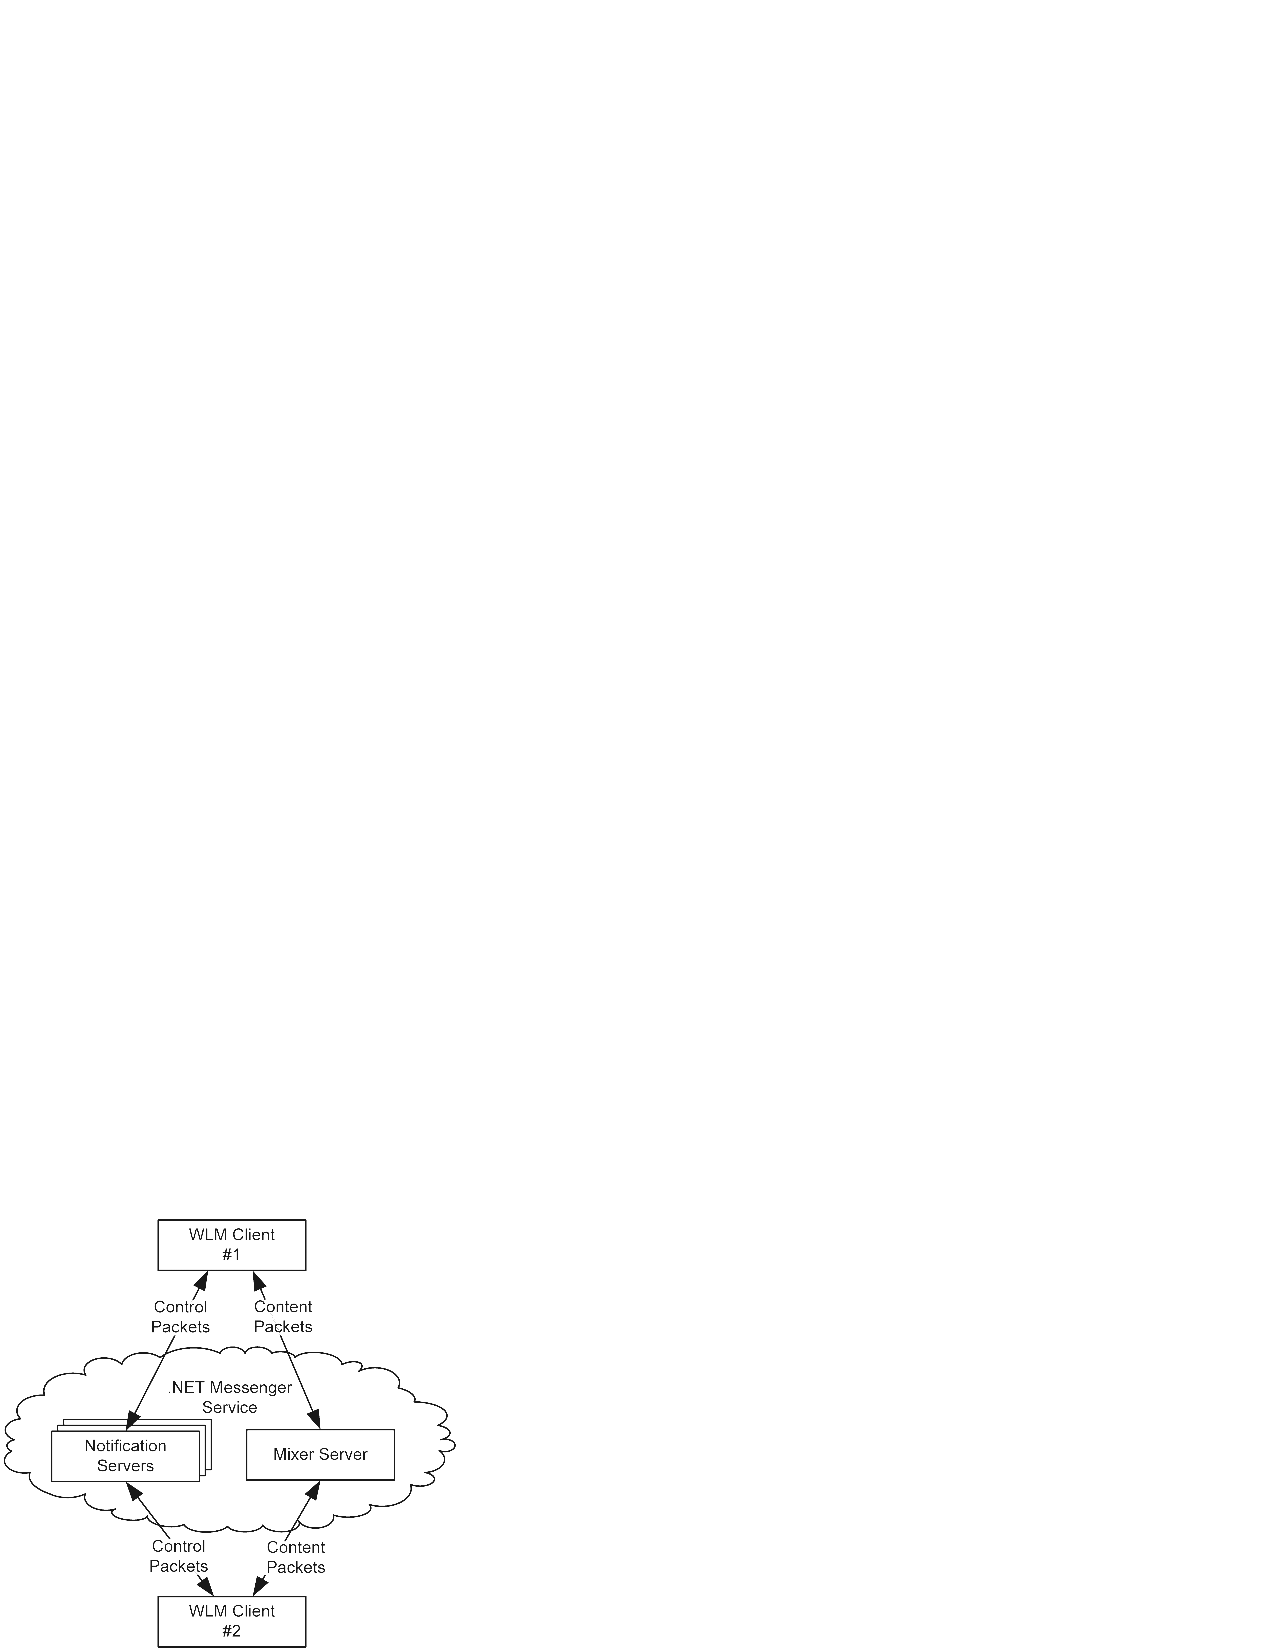
\includegraphics{graphics/infrastructure}
\end{figure}

When a user logs into their WLM account, a persistent TCP connection to an NS is established.
This connection must always remain active for the lifetime of the session; a lost connection will result in the client being logged out and disconnected from the messaging service.
Control packets are transmitted between the NS and the user via the persistent connection and include information such as a user's contact list and presence information (e.g., user status, email notification).

In addition to transmitting control packets, the NS also sends the client an IP address of the MS to be used for a new chat session.
For instance, if Alice attempts to talk to Bob, he will receive, from the connected NS, the location of an MS to which Bob needs to connect in order to chat with Alice.
Participants of an IM conversation are connected to the same MS, which relays content packets between clients.
These content packets carry messages, such as instant messages, sent among WLM clients through the mixer.

\subsection{Microsoft Notification Protocol}

MSNP is a text-based application protocol that defines the communication between WLM clients and servers.
Although the protocol was first intended to be an open standard~\cite{fout:insidewlm}, it has since become proprietary and has undergone numerous revisions.
However, due to the unencrypted nature of the protocol, attempts to reverse-engineer the protocol have proven successful~\cite{hypothetic:msnp, msnfanatic:msnp}.

The protocol consists of plain text commands; each command is prefixed with three capital letters (e.g., command \texttt{PNG} represents ping), and is sent in a separate packet.

To determine the validity of the persistent connection between the NS and the client, MSNP allows for asynchronous bidirectional pings; both the WLM client and the NS have the ability to initiate a ping.
The client pings the NS with \texttt{PNG}; the NS pings the client with \texttt{CHL}.
Both pings provoke responses from the receiving host. 
If a response is not received, the client will be disconnected from the messaging service.
WLM pings the NS every 45 seconds whereas in alternative IM clients, such as Pidgin~\cite{pidgin:url}, pings occur every 30 seconds.
Table~\ref{tab:commandlist} specifies the structure of MSNP commands that are relevant to our ABTH attack on MSNP.
Note that a ping initiated by the NS results in three MSNP commands (\texttt{CHL}-\texttt{QRY}-\texttt{QRY}).

Because confidentiality and integrity of MSNP traffic are not protected, an attacker can listen to the traffic and inject MSNP messages at will.
Afterwards, the attacker can employ ABTH and the MSNP commands shown in Table~\ref{tab:commandlist} to eliminate the discrepancy between the seqnums and acknums of the client and the NS created by the spoof packet.
Completion of ABTH will circumvent service disconnection and detection of a spoofed packet.
The fact that MSNP allows whitespace padding after commands can be leveraged to simplify ABTH calculations and reduce the number of packets necessary to resynchronize the TCP connection.

To illustrate our application of ABTH to MSNP, we describe in the following section how we have spoofed an MSNP command without disconnecting the client.
The spoofed command creates the effect of identity impersonation.

\subsection{Identity Spoofing}

\begin{table*}[tbp]
	\centering

	\caption{Identity spoofing sequence numbers}
	\label{tab:identityspoof}

	\begin{tabular}{l l l r r r r r}
		\hline
		\hline
		\textbf{Command} & \textbf{Sent By} & \textbf{Received By} & \textbf{Data Size} & \textbf{Client Seq} & \textbf{Client Ack} & \textbf{NS Seq} & \textbf{NS Ack} \\
		\hline
		\multicolumn{4}{l}{\textbf{Before Attack}} & 100 & 500 & 500 & 100 \\
		RNG & Attacker & Victim Client & 120 & 100 & \textbf{620} & 500 & 100 \\
		\multicolumn{8}{l}{\textbf{Begin ABTH}} \\
		PNG & Attacker & NS & 5 & 100 & 620 & 500 & \textbf{105} \\
		QNG & NS & Attacker & 8 & 100 & 620 & \textbf{508} & 105 \\
		\multicolumn{4}{l}{\textbf{Repeat PNG/QNG exchange for 23 more times \dots}} & 100 & 620 & \textbf{692} & \textbf{220} \\
		CHL & Attacker & Victim Client & 28 & 100 & \textbf{648} & 692 & 220 \\
		QRY & Victim Client & Attacker & 60 & \textbf{160} & 648 & 692 & 220 \\
		QRY & Attacker & Victim Client & 8 & 160 & \textbf{656} & 692 & 220 \\
		CHL & Attacker & Victim Client & 28 & 100 & \textbf{684} & 692 & 220 \\
		QRY & Victim Client & Attacker & 60 & \textbf{220} & 684 & 692 & 220 \\
		QRY & Attacker & Victim Client & 8 & 220 & \textbf{692} & 692 & 220 \\
		\hline
		\hline
		\multicolumn{4}{l}{\textbf{After ABTH}} & 220 & 692 & 692 & 220 \\
	\end{tabular}
\end{table*}

In order to accomplish an identity spoof, we will utilize the official WLM client, the live .NET Messaging Service, and a custom-made rogue WLM mixer server. 
The attacker injects a \texttt{RNG} command from the NS to the victim; this control packet is used by NS to invite the client to a new conversation session and contains two items of interest: the address of an MS and the email and name of the contact that invited the victim to the conversation.
The attacker can utilize these two parameters by setting the address of the MS to a rogue mixer server and setting the email and name of the user to impersonate.
Upon receiving the \texttt{RNG} command, the victim will connect to the specified MS to join an IM conversation with the user whose name and email was denoted in the command.

The injection of the \texttt{RNG} packet has caused the victim's acknum to grow by 120, the size of the \texttt{RNG}, and the victim's expected seqnum of the next TCP packet to increase by 120 as well.
As a result of this mismatch in the seqnums and acknums of the two hosts, further communication on this TCP connection will be dropped.
This mismatch can be resolved by utilizing ABTH to force the pretended source of the malicious packet, the NS, to actually send 120 bytes worth of data.
Forcing one side of the connection to send 120 bytes of data will also incur a cost in the sequence number space of the other side of the connection.
As a result, we will need to balance the seqnums and acknums of both sides of the connection to fill the 120 byte gap.
In the case of MSNP, we can use the \texttt{PNG}/\texttt{QNG} combination to inflate the NS side of the connection and the \texttt{CHL}/\texttt{QRY}/\texttt{QRY} combination to inflate the client.
Each \texttt{PNG}/\texttt{QNG} combination will elicit a cost of 8 bytes on the NS's seqnum and 5 bytes on the acknum.
The seqnum and acknum of client side of the connection can be increased via the \texttt{CHL}/\texttt{QRY}/\texttt{QRY} commands which will elicit a cost of 60 bytes to the client's seqnum and 36 bytes to the acknum.
With this information, we can form two algebraic equations where x represents the number of \texttt{PNG}/\texttt{QNG} combinations to send to the NS and y represents the number of \texttt{CHL}/\texttt{QRY}/\texttt{QRY} combinations to send to the client:

\begin{tabular}{ r l c l }
\((1)\) &   \(NS~seqnum\)    &   \(=\)    &\(Client~acknum\) \\
        &   \(5x\)           &   \(=\)    &\(60y\) \\
        &   \(x\)            &   \(=\)    &\(12y\) \\
\((2)\) &   \(Client~seqnum\)&   \(=\)    &\(NS~acknum\) \\
        &   \(8x\)           &   \(=\)    &\(36y+120\)
\end{tabular}

Putting these equations together, we get:

\begin{tabular}{ r c l }
\(8(12y)\)       &   \(=\)    &\(36y+120\) \\
\(\therefore y\) &   \(=\)    &\(2\) \\
\(\therefore x\) &   \(=\)    &\(24\)
\end{tabular}

As a result, we will need to inject 2 \texttt{CHL} commands to the client and 24 \texttt{PNG} commands to the NS.
Let us assume that prior to the spoofed packet, the seqnums of the client and the NS are 100 and 500, respectively, as shown in the first row of Table~\ref{tab:identityspoof}.
Each command is sent or received by the attacker in the order listed in Table~\ref{tab:identityspoof}.

As the last row shows, with matching seqnums and acknums, ABTH has successfully completed its series of application specific commands and has successfully resynchronized the TCP connection.
The connection is now is ready to transmit legitimate and/or illegitimate packets further.

As a result of spoofing the \texttt{RNG} command followed by synchronization using ABTH, the attacker is able to send/receive any number of IM chat messages to/from the victim, while impersonating the user specified in the \texttt{RNG} command.
As the victim's WLM client is unable to differentiate between a rogue mixer server and a legitimate one, it thereby cannot recognize the illegitimacy of the conversation.
From this point on, the attacker can continue his/her conversation with the victim until either the MS connection times out or the victim signs off.

\section{Discussion}
\label{sec:discussion}

Our experiments demonstrate that MSNP can be successfully attacked through ABTH.
However, ABTH has several caveats.

\subsection{Limitations}

In the case of WLM, it is crucial that ABTH is completed prior to the next client-to-NS ping, which occurs roughly every 45 seconds.
Otherwise, the client would ping the NS and discover the imbalance in seqnums, leading to a timeout and disconnection.
Depending on the resources of the attacker, ABTH can be reasonably accomplished within this timeframe, as our experiments---described in Section~\ref{sec:feasibility}---have demonstrated.

Our attack tool calculates and generates prior to the attack the required commands to send, which allows it to complete an attack within 2 seconds after it observes a \texttt{PNG} command sent from the victim to an NS.
If the victim's client and the NS exchange a packet during the restoration phase, ABTH would fail in resynchronizing their TCP stacks.
As a result, no network traffic can occur while ABTH is in progress. 
Our measurements described in Section~\ref{sec:feasibility} suggest that 2 seconds is a sufficiently short interval for achieving success rate of 95\%.
Complex algorithms capable of adjusting to live traffic dynamically might improve it further. 

ABTH requires the length of ping responses be greater than the commands issued to provoke them.
If this were not the case, an attempt to resynchronize the two hosts through ABTH would only widen the gap of mismatched seqnums.
Likewise, application commands that do not provoke responses would not work either, e.g., no operation or null data~\cite{joncheray:1995}.

\subsection{Countermeasures}

In order to properly authenticate messages, a naive countermeasure against ABTH is to encrypt all application traffic, for example with SSL/TLS.
However, WLM and other large-scale applications would require substantial server resources to encrypt all network traffic.
In the scenario where applications connect peers to peers by allowing a communication channel between two clients, as MSNP implicitly does through the mixer connection, clients may encrypt traffic and authenticate each other through the channel provided by the application.
For example, SimpLite-MSN~\cite{secway:url} sets up RSA keys and authenticates all instant messaging traffic for MSNP, thus providing protection against spoofing.

As ABTH requires a predetermined number of spoofed packets to inflate the seqnums and acknums of the hosts, intrusion detection systems (IDSs) may detect this form of attack due to the sudden spike in traffic between the hosts.
However, this behaviour may step within the boundaries of legitimate application traffic.

Furthermore, a regulatory mechanism in the application protocol, such as tagging application messages with sequence numbers, has the potential for providing integrity for each packet.
With such a mechanism, it would be difficult to inject a packet and expect further messages to be accepted.
This straightforward yet non-trivial detail also alleviates the application protocol from its dependence on the network layer and the assumption that packets on the network layer are authentic.

For network service providers, the most effective method to disable ABTH and message spoofing altogether would be to prohibit IP packets with forged source IP addresses~\cite{templeton:spoof}.
However, this method would be ineffective in an unencrypted wireless medium, such as WiFi, commonly found in coffee shops and other public locations. 

\vfil\eject

\subsection{Feasibility}
\label{sec:feasibility}

Our implementation of ABTH on MSNP completes within roughly 2 seconds and is triggered on the reception of a MSNP \texttt{PNG} command.
In order for the attack to succeed, no message exchange between the victim's client and the NS can occur within these 2 seconds.
While the amount of MSNP traffic is dependent on a variety of factors, we logged the success rate against the number of online WLM contacts, which is the only quantifiable metric in a WLM session.
Our measurements obtained through monitoring several days of MSNP traffic suggest that the probability of a control message occurring within 2 seconds of a ping is less than 5\%, regardless of the number of contacts online on the contact list, as can be seen in Figure~\ref{fig:successrate}.

\begin{figure}[h]
	\centering
	\caption{Success rate of ABTH attack vs. the number of victim's contacts being online.}
	\label{fig:successrate}
	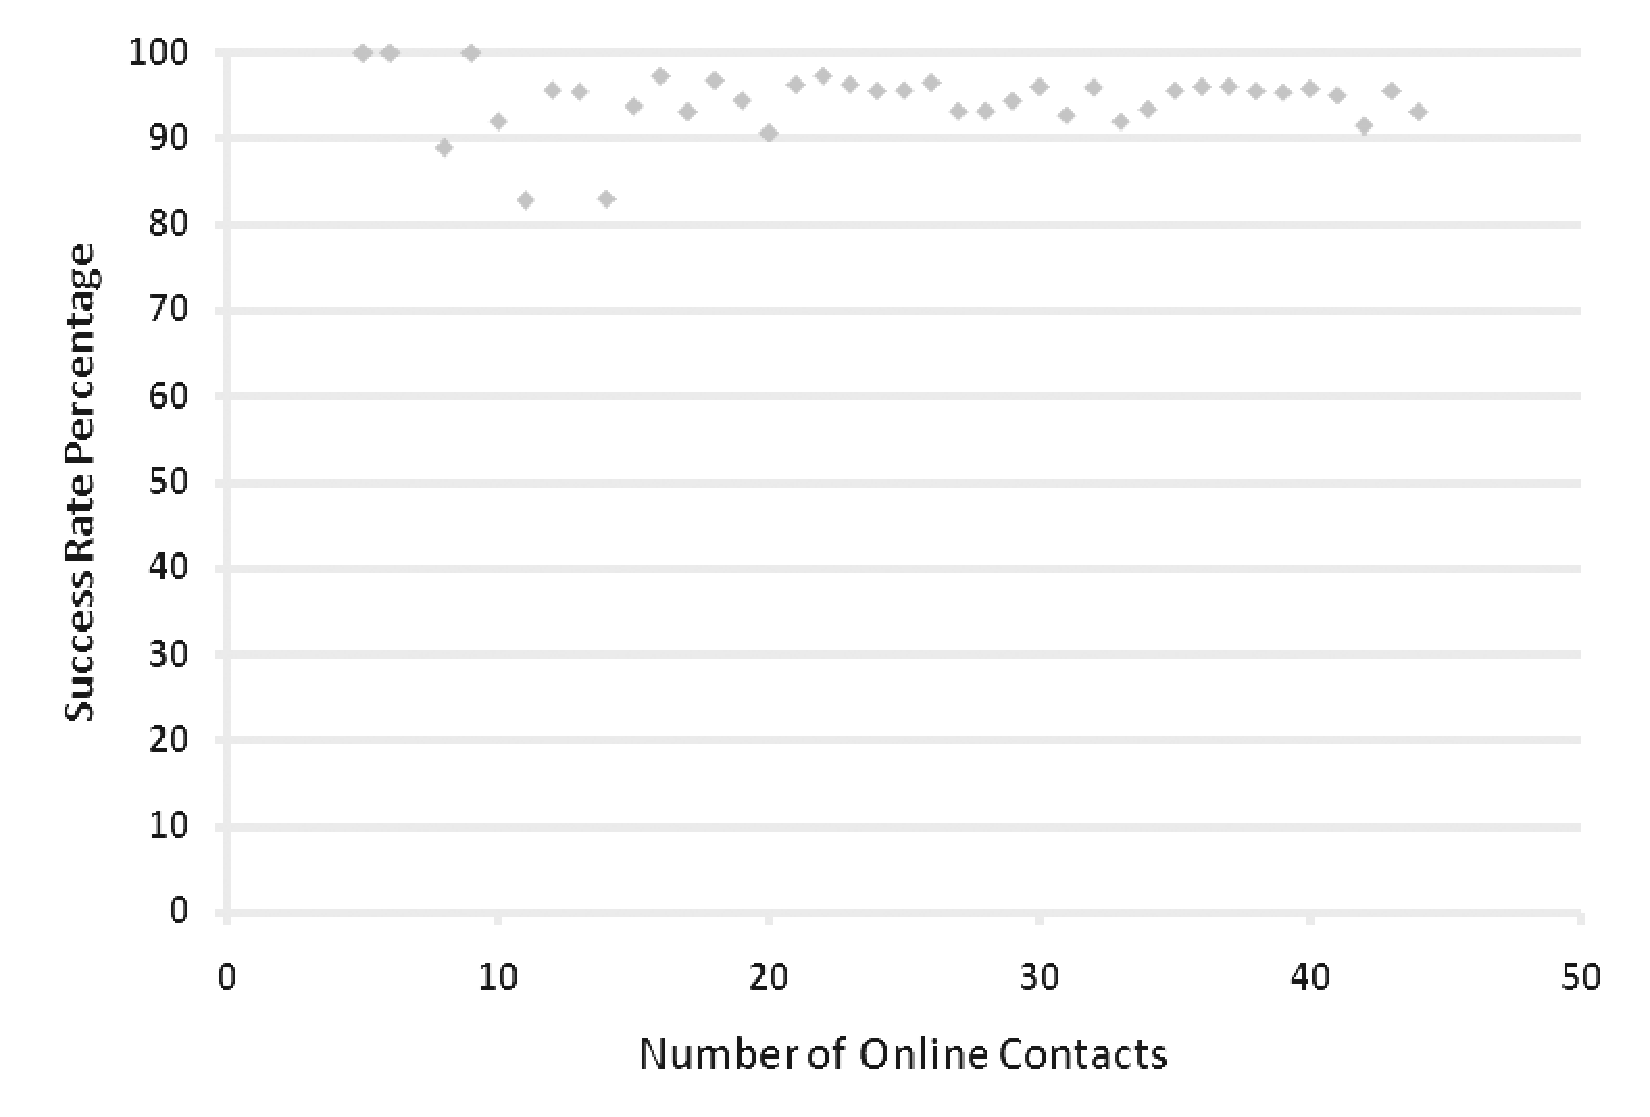
\includegraphics[width=\columnwidth]{graphics/plot}
\end{figure}

\subsection{Victim Environment}
\label{sec:victimenvironment}

The implementation of the TCP/IP stack on the victim's operating system dictates the behaviour of an ABTH attack.
The quirk is that different implementations behave differently upon receiving a packet with unexpected seq and acknums.
Gathered from empircal tests, we summarize three TCP stacks in Table~\ref{tab:implementations}: an ideal (non-existent) RFC specified interpretation of TCP packet processing (as shown in~\cite{zaghal:model}), and the TCP stack implementation on Microsoft Windows and on Linux.
These only deal with packets with seqnum within the acceptable range (greater or equal to expected seqnum and smaller than the receive window); otherwise, the packet is dropped and an ack is sent back regardless of the implementation of the TCP stack.

\begin{table*}[tbp]
	\centering

	\caption {Treatment of a packet with unexpected seqnums and acknums on different TCP stacks}
	\label{tab:implementations}

	\begin{tabular}{c|c|c|c|c|c|c|c}
		\hline
		\textbf{Seqnum} & \textbf{Acknum} & \multicolumn{2}{|c|}{\textbf{RFC Specified Interpretation}} & \multicolumn{2}{|c|}{\textbf{Microsoft Windows}} & \multicolumn{2}{|c}{\textbf{Linux}} \\
		& & Accepted & Ack Returned & Accepted & Ack Returned & Accepted & Ack Returned \\
		\hline
		= Expected & $\leq$ Expected & $\checkmark$ & $\checkmark$ & $\checkmark$ & $\checkmark$ & $\checkmark$ & $\checkmark$ \\
		\hline
		= Expected & $>$ Expected & $\times$ & $\checkmark$ & $\times$ & $\checkmark$ & $\checkmark$ & $\checkmark$ \\
		\hline
		$>$ Expected & $\leq$ Expected & $\checkmark$ & $\times$ & $\checkmark$ & $\times$ & $\checkmark$ & $\times$ \\
		\hline
		$>$ Expected & $>$ Expected & $\times$ & $\checkmark$ & $\times$ & $\times$ & $\times$ & $\checkmark$ \\
		\hline
	\end{tabular}

	\begin{flushleft}
		The $>$ Expected value for Seqnum implies that the number is larger than the expected value but smaller than the receive window, thus falling within range of acceptable seqnum.
	\end{flushleft}
\end{table*}

In the RFC specified interpretation, each ping packet, \texttt{PNG} in the case of MSNP, would be met with an additional ack storm.
In a publicly switched network where packet latency is typically 20ms, the MSNP ABTH attack that takes 2 seconds would generate roughly 2500 ack packets, assuming the attacker generates a packet every round trip time (40ms).
Whether or not this statistic is acceptable for a TCP attack based on its environment and threat model is beyond the scope of this discussion, although we believe this is quite low.

In the Windows implementation, which was used extensively in our testing, no acks are returned for packets with seqnums and acknums larger than the expected (row 4 of Table~\ref{tab:implementations}).
This directly resulted in elimination of ack storms all together; a total of two ack packets are sent by the victim.
Our assumption in this case is that the NS of the .Net Messenger Service runs on Windows.

In the case of Linux, the attack fails completely.
Since a packet with the expected seqnum but larger than expected acknum (row 2 of Table~\ref{tab:implementations}) is accepted by the TCP stack, it renders complete descynchronization quite difficult.
The host that receives response packets, \texttt{QNG} in the case of MSNP, would accept them and pass them to the application.
Any attempt to elicit response to fill a gap in seqnum (caused by a malicious packet) would increase the acknum of the receiving host, and thus fail.

\section{Conclusion}
\label{sec:conclusion}

By exploiting a combination of the innocuous features of the transport and application layers and by taking advantage of the lack of confidentiality and integrity protection at either layer, application-based TCP hijacking (ABTH) offers an elegant way of attacking certain application protocols.
Sending commands to both hosts to provoke responses allows an attacker to create a gap in TCP sequence numbers of a size exactly large enough for the injection of a spoofed command.
We presented a proof of the ABTH concept by successfully applying it to attack Windows Live Messenger, Microsoft's popular instant messaging application, which uses the Microsoft Notification Protocol (MSNP).

While some protocols, such as MSNP, were designed to suit flexible environments, as the environment evolved, these features have become subtle vulnerabilities.
Although hardware Ethernet equipment has been updated to obstruct lower level attacks (e.g., ARP poisoning), the realm of attacks is reaching beyond the protection capabilities of network devices.
In environments that provide a common physical communication medium, such as hubbed networks and coffee shops that offer unencrypted WiFi service, ABTH poses a threat.
Application protocols vulnerable to ABTH, such as MSNP, were not designed to offer secure communication channels.
As such, it is imperative that, as protocols become more widely adopted, they are improved upon and revised to accommodate their broadening uses.

\vfil\eject

\bibliographystyle{abbrv}
\bibliography{abthmsnp}

\end{document}
